\documentclass{article}

\usepackage{tikz}
\usetikzlibrary{automata, positioning}
\begin{document}
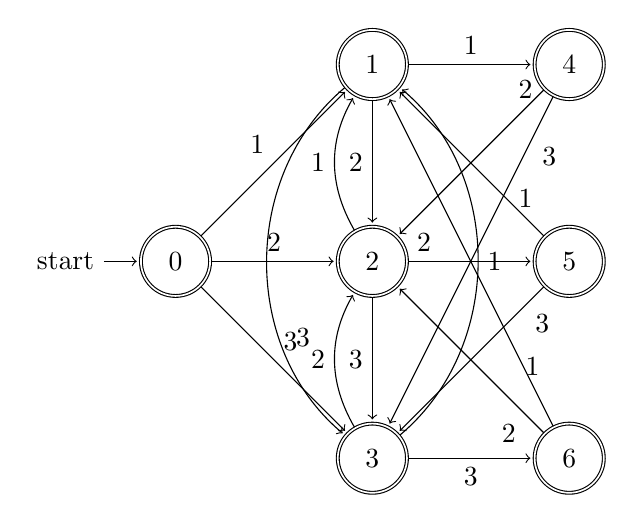
\begin{tikzpicture}[shorten >= 1pt, node distance = 2.5cm, on grid, auto]
  \node[state, initial, accepting] (0) {0};
  \node[state, accepting] (2) [right=of 0] {2};
  \node[state, accepting] (1) [above=of 2] {1};
  \node[state, accepting] (3) [below=of 2] {3};
  \node[state, accepting] (4) [right=of 1] {4};
  \node[state, accepting] (5) [right=of 2] {5};
  \node[state, accepting] (6) [right=of 3] {6};
  \path[->]
    (0) edge node {1} (1)
        edge node {2} (2)
        edge node {3} (3)
    (1) edge node [left] {2} (2)
        edge [bend right=50] node [near end] {3} (3)
        edge node {1} (4)
    (2) edge node [left] {3} (3)
        edge [bend left] node [left] {1} (1)
        edge node [very near start] {2} (5)
    (3) edge [bend left] node [left] {2} (2)
        edge [bend right=50] node [right] {1} (1)
        edge node [below] {3} (6)
    (4) edge node [very near start, above] {2} (2)
        edge node [very near start] {3} (3)
    (5) edge node [very near start] {3} (3)
        edge node [very near start, above] {1} (1)
    (6) edge node [very near start] {2} (2)
        edge node [very near start, above] {1} (1);
\end{tikzpicture}
\end{document}
